\documentclass[]{book}
\usepackage{lmodern}
\usepackage{amssymb,amsmath}
\usepackage{ifxetex,ifluatex}
\usepackage{fixltx2e} % provides \textsubscript
\ifnum 0\ifxetex 1\fi\ifluatex 1\fi=0 % if pdftex
  \usepackage[T1]{fontenc}
  \usepackage[utf8]{inputenc}
\else % if luatex or xelatex
  \ifxetex
    \usepackage{mathspec}
  \else
    \usepackage{fontspec}
  \fi
  \defaultfontfeatures{Ligatures=TeX,Scale=MatchLowercase}
    \setmainfont[]{Libre Baskerville}
    \setmonofont[Mapping=tex-ansi]{Fantasque Sans Mono}
\fi
% use upquote if available, for straight quotes in verbatim environments
\IfFileExists{upquote.sty}{\usepackage{upquote}}{}
% use microtype if available
\IfFileExists{microtype.sty}{%
\usepackage[]{microtype}
\UseMicrotypeSet[protrusion]{basicmath} % disable protrusion for tt fonts
}{}
\PassOptionsToPackage{hyphens}{url} % url is loaded by hyperref
\usepackage[unicode=true]{hyperref}
\PassOptionsToPackage{usenames,dvipsnames}{color} % color is loaded by hyperref
\hypersetup{
            pdftitle={Internship Report},
            pdfauthor={Subham Roy},
            colorlinks=true,
            linkcolor=Maroon,
            citecolor=Blue,
            urlcolor=Blue,
            breaklinks=true}
\urlstyle{same}  % don't use monospace font for urls
\usepackage[bottom=1.25in,a4paper]{geometry}
\usepackage{longtable,booktabs}
% Fix footnotes in tables (requires footnote package)
\IfFileExists{footnote.sty}{\usepackage{footnote}\makesavenoteenv{long table}}{}
\usepackage{graphicx,grffile}
\makeatletter
\def\maxwidth{\ifdim\Gin@nat@width>\linewidth\linewidth\else\Gin@nat@width\fi}
\def\maxheight{\ifdim\Gin@nat@height>\textheight\textheight\else\Gin@nat@height\fi}
\makeatother
% Scale images if necessary, so that they will not overflow the page
% margins by default, and it is still possible to overwrite the defaults
% using explicit options in \includegraphics[width, height, ...]{}
\setkeys{Gin}{width=\maxwidth,height=\maxheight,keepaspectratio}
% Make links footnotes instead of hotlinks:
\renewcommand{\href}[2]{#2\footnote{\url{#1}}}
\IfFileExists{parskip.sty}{%
\usepackage{parskip}
}{% else
\setlength{\parindent}{0pt}
\setlength{\parskip}{6pt plus 2pt minus 1pt}
}
\setlength{\emergencystretch}{3em}  % prevent overfull lines
\providecommand{\tightlist}{%
  \setlength{\itemsep}{0pt}\setlength{\parskip}{0pt}}
\setcounter{secnumdepth}{5}
% Redefines (sub)paragraphs to behave more like sections
\ifx\paragraph\undefined\else
\let\oldparagraph\paragraph
\renewcommand{\paragraph}[1]{\oldparagraph{#1}\mbox{}}
\fi
\ifx\subparagraph\undefined\else
\let\oldsubparagraph\subparagraph
\renewcommand{\subparagraph}[1]{\oldsubparagraph{#1}\mbox{}}
\fi

% set default figure placement to htbp
\makeatletter
\def\fps@figure{htbp}
\makeatother

\usepackage{subfig}
\AtBeginDocument{%
\renewcommand*\figurename{Figure}
\renewcommand*\tablename{Table}
}
\AtBeginDocument{%
\renewcommand*\listfigurename{List of Figures}
\renewcommand*\listtablename{List of Tables}
}
\usepackage{float}
\floatstyle{ruled}
\makeatletter
\@ifundefined{c@chapter}{\newfloat{codelisting}{h}{lop}}{\newfloat{codelisting}{h}{lop}[chapter]}
\makeatother
\floatname{codelisting}{Listing}
\newcommand*\listoflistings{\listof{codelisting}{List of Listings}}

\title{Internship Report}
\author{Subham Roy}
\providecommand{\institute}[1]{}
\institute{PEC University of Technology}
\date{January 20, 2014}

\begin{document}
\maketitle

{
\hypersetup{linkcolor=black}
\setcounter{tocdepth}{2}
\tableofcontents
}
\pagenumbering{arabic} \listoffigures

\chapter{Summary}\label{summary}

During my internship period at STMicroelectronics, Greater Noida, India,
I was involved with several projects in the AMG\footnote{Analog and MEMS Group}
Systems Lab Department and in the S\&M Department. The AMG Systems Lab,
also called the Central Lab, is involved with the design, development
and implementation of various proof-of-concept systems revolving around
fields like IoT, LED lighting, efficient power supplies, wireless
communication systems and various motor control applications. As part of
the S\&M Department and AMG Systems Lab, I got an oppurtunity to work on
various realms of the industry, from application software development
and firmware development to circuit design and testing. A brief
categorisation of the projects is depicted in
figure~\ref{fig:proj_categ}. A short summary of each project is also
mentioned in section~\ref{sec:proj_sum}.

\begin{figure}
\centering
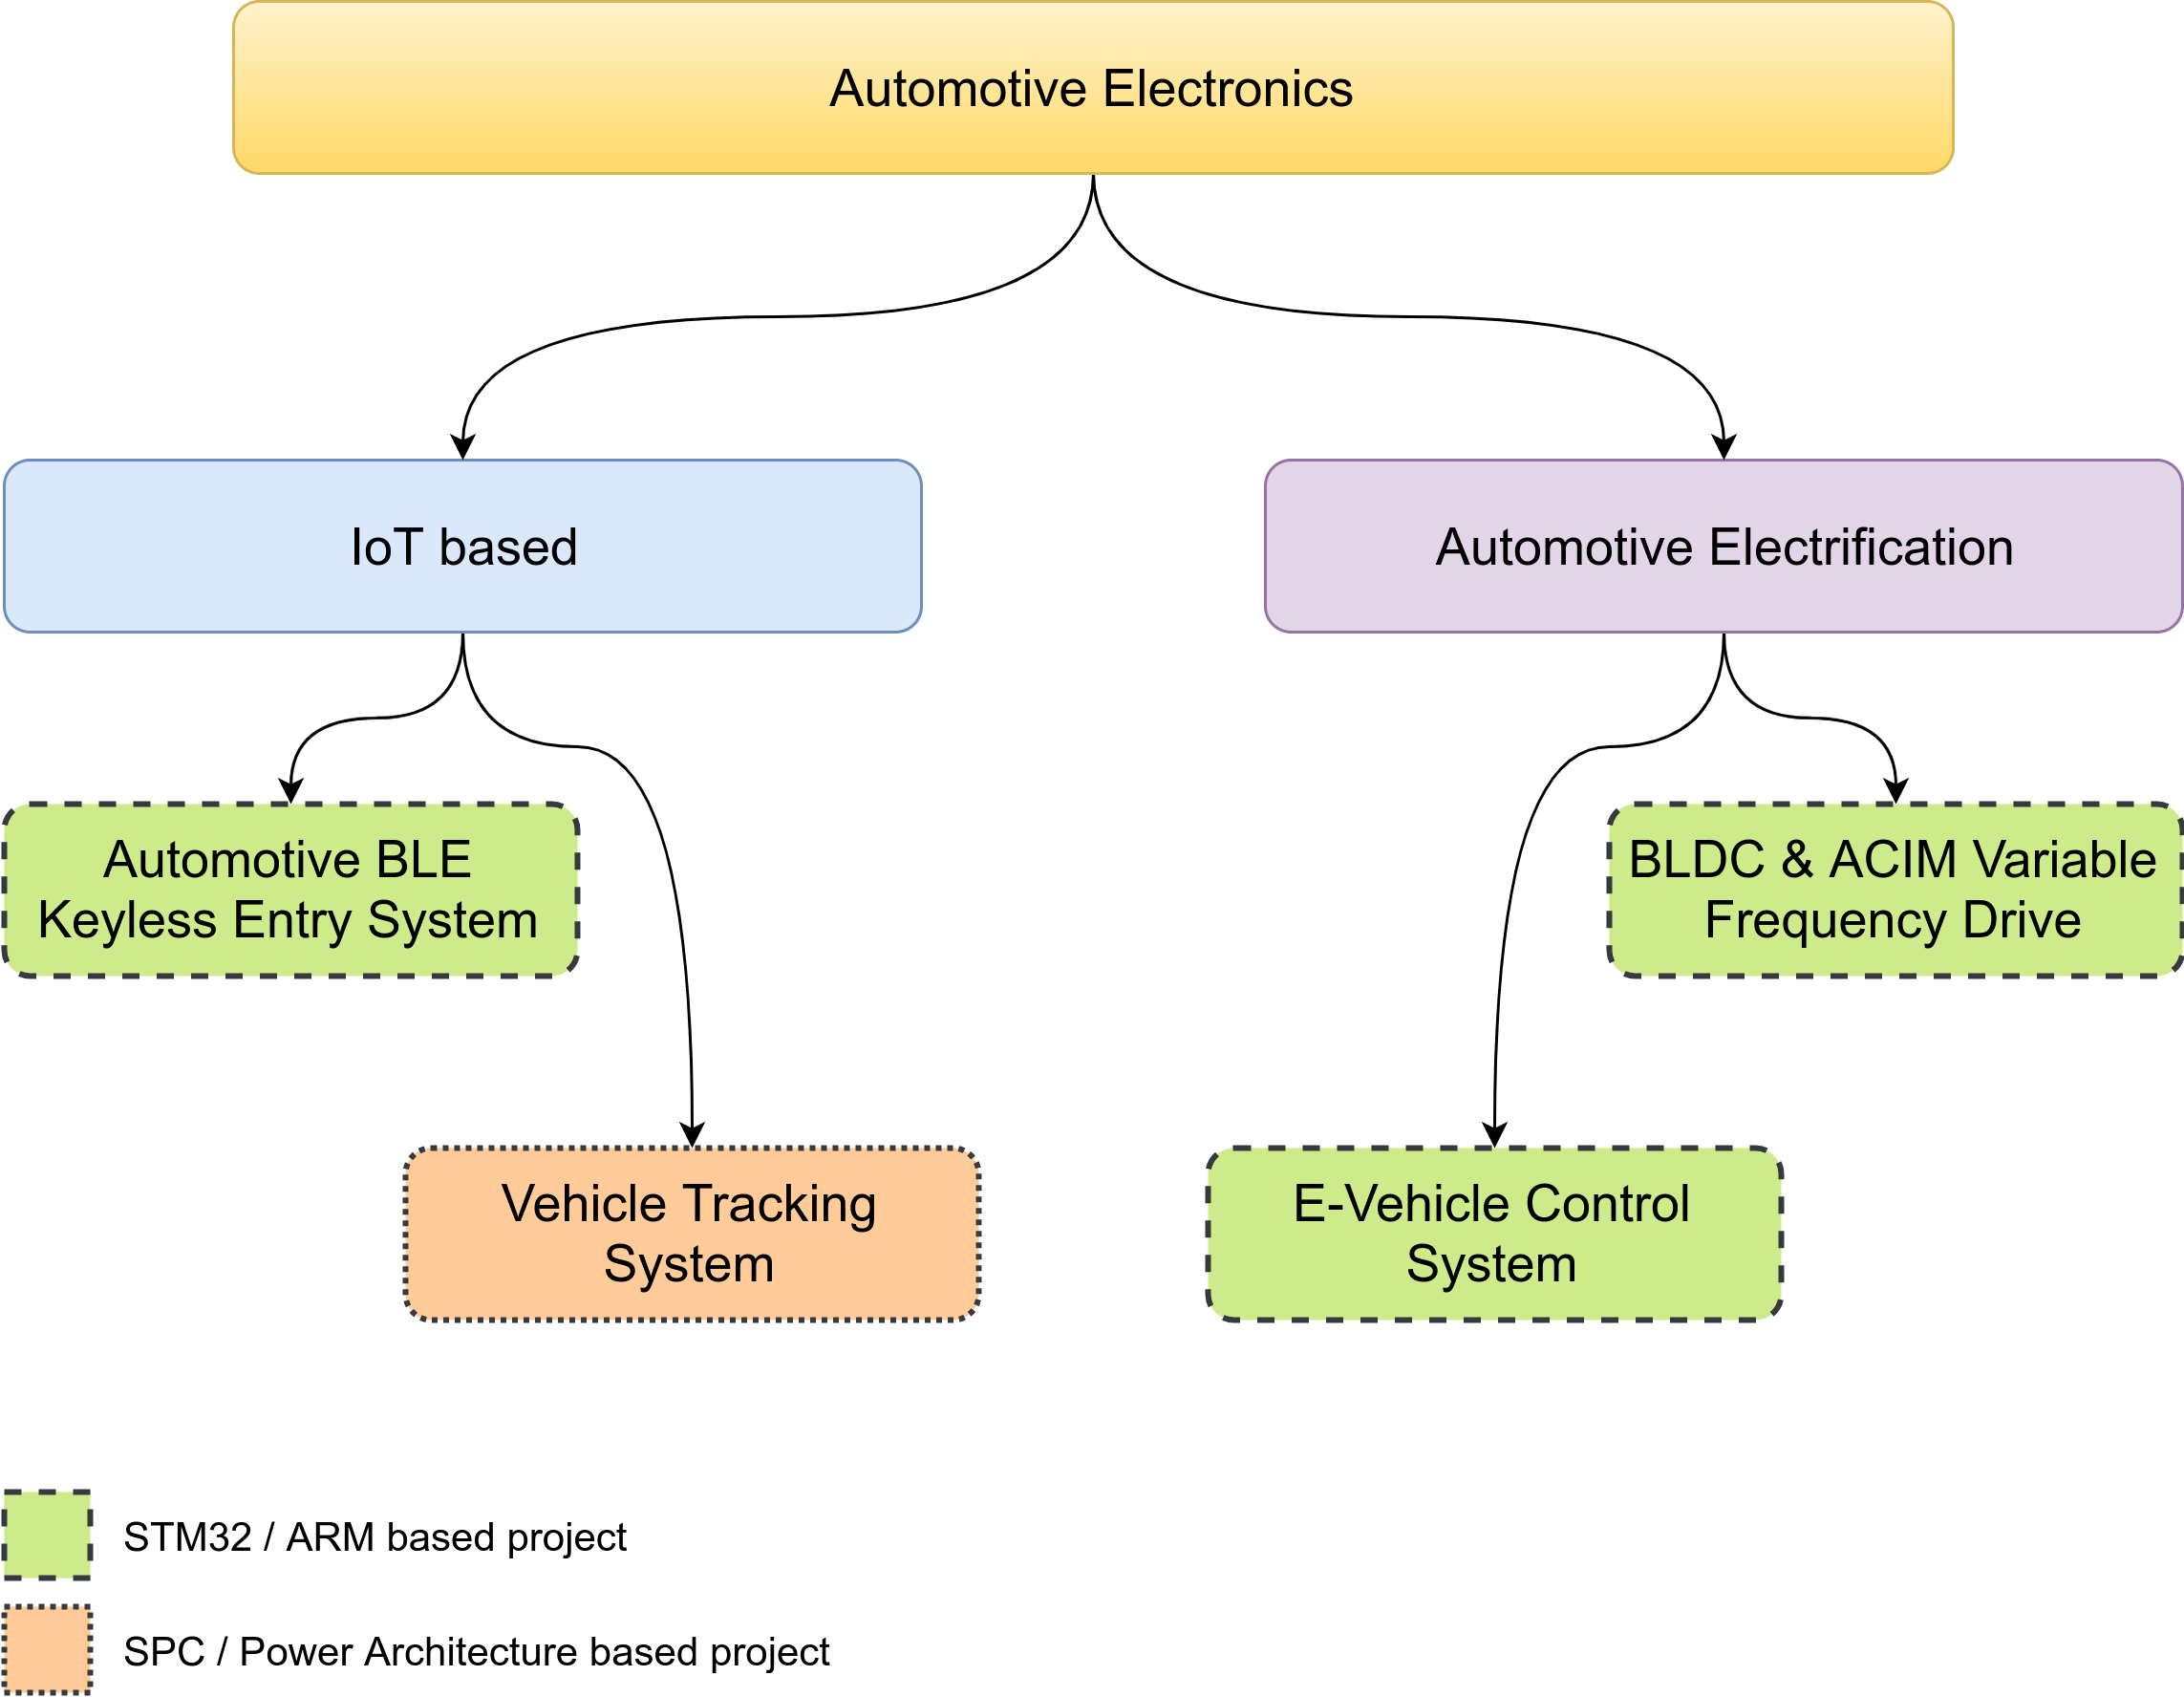
\includegraphics{img/proj_categ.png}
\caption{Categorisation of projects done in the Internship
period.}\label{fig:proj_categ}
\end{figure}

\section{Summary of projects}\label{sec:proj_sum}

This is a summary of the broad fields and the corresponding projects
that I was involved with in STMicroelectronics, India.

\subsection[BLDC and ACIM Drives and Speed
Controllers]{\texorpdfstring{BLDC\footnote{Brush-less DC} and
ACIM\footnote{AC Induction Motor} Drives and Speed
Controllers}{BLDC and ACIM Drives and Speed Controllers}}\label{sec:bldc_sum}

Electrical motors are one of the most used actutators that can convert
electrical energy to mechanical energy. Many other mechanical actuators
like the Hydraulic Cylinder is a linear actuator, which has , electrical
motors deliver mechanical energy in the form of rotation.

PMSM,\footnote{Permanant Magnet Synchronous Motor} are synchronous
motors that use permanant magnets for magnetic field generation instead
of a separate set of windings called the field windings. BLDC motors are
a special kind of PMSM, also called the ECM or
Electronic Commutation Motor. These are called so, because, instead of
having a mechanical commutator\footnote{Mechanical commutators are
  common in electrical machines like the permanant magnet DC motor.}, a
specifically conditioned signal is provided to the windings
directly\footnote{later discussed in section~\ref{sec:bldc_motors}}. The
electronic device which is responsible for the generation of such a
conditioned signal, for the BLDC motor is called a \emph{BLDC Motor
Drive}.

Following is a brief list about the projects involving BLDC and ACIM
motor drives.

\begin{itemize}
\item
  \textbf{BLDC Motor Drive on SPC platform} : The project involved
  testing of a BLDC drive library already implemented by
  STMicroelectronics. An exhaustive testing and verification of the
  firmware library was done.
\item
  \textbf{BLDC Motor Drive on STM8 platform}: This involved design and
  tuning of the motor drive using the six-step commutation algorithm.
  Although, the Motor Drive power stage (MB459) was designed for both
  low voltage (\textless{}35V) and high voltage(\textgreater{}35V)
  operations but the end objective was to drive a high power BLDC motor
  at 48V. The peak power rating of the motor drive was around 300W. The
  motor drive features Over current protection, over voltage protection,
  BEMF sampling, Configurable one or three shunt Current Sensing,
  Configurable UI and user input options and regenerative braking
  ability. The Motor Drive controls speed through a PI controller and
  can perform torque regulation in closed loop operation.
\item
  \textbf{ACIM drive on STM32 (STM32F303RE)} : This involved porting of
  an already implemented firmware from one Hardware Abstraction Layer
  (STM32-ARM Standard Peripheral Lib) to another (STM32 Cube HAL).
\end{itemize}

\subsection{Automotive Keyless Entry System using
BLE}\label{automotive-keyless-entry-system-using-ble}

The objective of this project was to implement a communication system
between a mobile phone app and a BlueNRG1 hardware module to transmit
character messages. The BlueNRG1 is a dedicated SoC\footnote{System on Chip}
for Bluetooth applications. This project was designed for an automotive
application in which the mobile app is used to unlock or lock an
automobiles central locking system.

\subsection{Vehicle Tracking System}\label{vehicle-tracking-system}

IoT is a fast expanding field for electronics devices. Many technologies
and protocols have been developed and rigorously tested to expand the
notion of internet onto devices like LED lighting systems, household
security and surveillance systems. Technologies such as
6LoWPAN\footnote{\textbf{6LowPan} is an abbreviation for IPv6 over Low
  power Wireless Personal Area Networks. It is a technology that was
  originally intended to extend internet connectivity to smaller low
  power devices that may not have any dedicated TCP/IP stack.
  Now-a-days, it is used for creating pico-nets or micro-networks of
  devices, +P2P!! device communication.} are aimed at connecting even
the smallest of electronic devices like discrete sensor units and
household objects. The idea of IoT in household objects is quite
interesting. One such application was the use of RFID technology to
detect the location of small household objects like keys. The Vehicle
Tracking System is an attempt to bring IoT technology to automobiles.
The Vehicle Tracking System involves a hardware module incorporated in
an automobile and a central server system, designed to transmit and
store data in the cloud(central server), which can be accessed by the
user via an Android app. The objective was to design and implement a
hardware module. The hardware module comprised of a micro-controller
(SPC560D40L1) and a GSM module (Quectel M66). The hardware module uses
the GSM communication band to transmit vital automobile statistics to
the central server via the TCP/IP data packeting protocol. HTTP was used
at the application layer.

\subsection{Implementation of Servo Motor Abstraction
library.}\label{implementation-of-servo-motor-abstraction-library.}

A hardware abstraction library for servo motors was implemented using
STM32 Cube HAL on STM32F3 platform. The Servo library featured APIs for
setting the Servo final position and the speed of rotation.

\chapter{Introduction}\label{introduction}

\section{TODO : brief intro about automotive
industry}\label{todo-brief-intro-about-automotive-industry}

\section{Battery technology in Automotive
Industry}\label{battery-technology-in-automotive-industry}

The automotive industry is expanding at a rapid pace. Automobiles are
now-a-days more ``smarter'' and react to environment changes more
rapidly. Contrast todays vehicles with the first ever automobiles, which
had no logical processing units or sensors. Everything needed to done
manually. Today, autmotive industry is highly dependent on the
electronics industry for providing efficient systems. This may be called
\textbf{Automotive Electrification}. With the introduction of
high-efficiency high-density LiPo\footnote{LiPo is an abbreviation for
  Lithium-Polymer ion batteries. These are a variety of battery which
  uses a polymer electrolyte composed of Li ions instead of a
  traditional liquid electrolyte. These are extremely light weight and
  pack a relatively larger amount of energy per volume than other types
  available.} batteries in the market, the automotive market has taken a
turn towards electrification of vehicles. Corporations like Tesla Motors
are the pioneers of this technology. With an increase in the production
of various kinds of cells and batteries, the market has been flooded
with these components. As a consequence, the prices for batteries has
dropped sharply in the last decade. This has also impacted the
automotive industry, with big companies like Tesla Motors to take the
intitiative for making ``clean'' and pollution-free vehicles. Due to the
reduced costs and a foresee-able future of such components, developing
countries like India has also started embracing this technology.
Introduction of light battery-powered three and four wheelers on Indian
roads is a direct consequence of this trend.

\section{Internet of Things}\label{internet-of-things}

Internet of Things refers to a network of physical objects, like
household articles, vehicles, tools, buildings, worn-items, etc.
embedded with suitable software and hardware. This software and hardware
may enable these objects to communicate with each other or with devices
on another network like the Internet. IoT\footnote{+IoT!!} is also a
rapidly growing field. Wireless IoT devices are now-a-days avaialable in
any shape or size, starting from smart household appliances like TV, AC,
Refrigerators, etc. to small beacons the size of a coin and wearable
devices. IoT enabled devices may enable the user to interact with the
devices in a number of ways, which include:

\begin{itemize}
\tightlist
\item
  Controlling the device with the help of another device like a mobile
  phone or a computer.
\item
  Controlling the device with help of HID (Human Interface Device).
\item
  Controlling the device with the help of ones body, using suitable
  sensors. For example, a smart-watch may be used to turn on an
  appliance when it detects motion in a certain direction. Sensors such
  as accelerometers and gyroscopes may be used to detect linear or
  radial motion.
\item
  Device controlling another appliance.
\end{itemize}

The uses of IoT are limitless and it is just a matter of time, when the
market will be flooded with IoT based devices.

\section{Combining Automotive Electrification and
IoT}\label{combining-automotive-electrification-and-iot}

With the development of dedicated sensors and low cost IoT devices, it
is now possible to efficiently integrate IoT into automobiles. Various
kinds of electronic integration is already existent in present
automobiles, such as

\begin{itemize}
\tightlist
\item
  \textbf{Automotive ECU} : ECU stands for Engine Control Unit. It is a
  logical control system, which takes some input data from the
  automobiles engine sensors like temperature, acceleration, rate of
  fuel flow, etc. The ECU is responsible for the efficient combustion of
  fuel and maintaining the engine conditions well within its operation
  limits.
\item
  \textbf{Body Control Devices} : Body Control Units are responsible for
  various body control functions of the automobile like central locking
  system, power windows, various lights like the headlights, tail-lights
  and indicator lights.
\item
  \textbf{Automotive Audio Equipment} : Audio Equipments in automobiles
  are composed of various electronic devices like audio amplifiers,
  radio-frequency systems, audio decoders and effects-processors(DSP),
  low noise amplifiers, speaker systems.
\item
  \textbf{CAN Bus} : CAN stands for Controller Area Network. It is a
  automotive bus specification designed for high speed data transfer.
  The CAN bus enables several microcontrollers to share data with each
  other without the presence of a host or central system. It is used for
  integrating various electronic automotive components like the ECU,
  Body control unit, sensors, etc. with each other so that they can
  function in harmony. The CAN bus is discussed in more detail in
  \{section~\ref{sec:canbus}\}
\end{itemize}

\subsection{The need for IoT in
automobiles}\label{the-need-for-iot-in-automobiles}

\begin{itemize}
\tightlist
\item
  Integration of more and more Silicon\footnote{Silicon, here refers to
    electronic logic components. These may refer to logic gates, ASICs,
    sensors or microcontroller units.} into automobiles.
\item
  Smarter and more efficient automobiles.
\item
  Larger economic benefit. Smarter automobiles are more desirable in the
  current market and hence provide more economic value than its
  counterparts.
\end{itemize}

\chapter{Software Tools and Hardware Components}\label{sec:tools}

\begin{longtable}[]{@{}lll@{}}
\caption{A brief summary of the tools used, look
table~\ref{tbl:my_tble}}\tabularnewline
\toprule
\begin{minipage}[b]{0.13\columnwidth}\raggedright\strut
Specifications\strut
\end{minipage} & \begin{minipage}[b]{0.13\columnwidth}\raggedright\strut
Title\strut
\end{minipage} & \begin{minipage}[b]{0.64\columnwidth}\raggedright\strut
Justification\strut
\end{minipage}\tabularnewline
\midrule
\endfirsthead
\toprule
\begin{minipage}[b]{0.13\columnwidth}\raggedright\strut
Specifications\strut
\end{minipage} & \begin{minipage}[b]{0.13\columnwidth}\raggedright\strut
Title\strut
\end{minipage} & \begin{minipage}[b]{0.64\columnwidth}\raggedright\strut
Justification\strut
\end{minipage}\tabularnewline
\midrule
\endhead
\begin{minipage}[t]{0.13\columnwidth}\raggedright\strut
Operating Sytem\strut
\end{minipage} & \begin{minipage}[t]{0.13\columnwidth}\raggedright\strut
Windows 7\strut
\end{minipage} & \begin{minipage}[t]{0.64\columnwidth}\raggedright\strut
Base OS\strut
\end{minipage}\tabularnewline
\begin{minipage}[t]{0.13\columnwidth}\raggedright\strut
IDE\strut
\end{minipage} & \begin{minipage}[t]{0.13\columnwidth}\raggedright\strut
IAR Workbench\strut
\end{minipage} & \begin{minipage}[t]{0.64\columnwidth}\raggedright\strut
IDE for ARM embedded software development\strut
\end{minipage}\tabularnewline
\begin{minipage}[t]{0.13\columnwidth}\raggedright\strut
IDE\strut
\end{minipage} & \begin{minipage}[t]{0.13\columnwidth}\raggedright\strut
SPC5Studio\strut
\end{minipage} & \begin{minipage}[t]{0.64\columnwidth}\raggedright\strut
IDE for SPC embedded software development\strut
\end{minipage}\tabularnewline
\begin{minipage}[t]{0.13\columnwidth}\raggedright\strut
Software\strut
\end{minipage} & \begin{minipage}[t]{0.13\columnwidth}\raggedright\strut
UDE Debugger Toolkit\strut
\end{minipage} & \begin{minipage}[t]{0.64\columnwidth}\raggedright\strut
A debugger software that supports debugging of microcontrollers with the
IEEE compliant JTAG specifications\strut
\end{minipage}\tabularnewline
\begin{minipage}[t]{0.13\columnwidth}\raggedright\strut
Software\strut
\end{minipage} & \begin{minipage}[t]{0.13\columnwidth}\raggedright\strut
STM32 CubeMX\strut
\end{minipage} & \begin{minipage}[t]{0.64\columnwidth}\raggedright\strut
Firmware Code Generator for the STM32 ARM hardware platform
devices\strut
\end{minipage}\tabularnewline
\begin{minipage}[t]{0.13\columnwidth}\raggedright\strut
API\strut
\end{minipage} & \begin{minipage}[t]{0.13\columnwidth}\raggedright\strut
BlueNRG-DK\strut
\end{minipage} & \begin{minipage}[t]{0.64\columnwidth}\raggedright\strut
A comprehensive software development kit for the BlueNRG family of
SoCs\strut
\end{minipage}\tabularnewline
\begin{minipage}[t]{0.13\columnwidth}\raggedright\strut
Programming Language\strut
\end{minipage} & \begin{minipage}[t]{0.13\columnwidth}\raggedright\strut
C\strut
\end{minipage} & \begin{minipage}[t]{0.64\columnwidth}\raggedright\strut
Default language interface for IAR and ppc-gcc-vle compilers used in
code production\strut
\end{minipage}\tabularnewline
\begin{minipage}[t]{0.13\columnwidth}\raggedright\strut
Hardware Device\strut
\end{minipage} & \begin{minipage}[t]{0.13\columnwidth}\raggedright\strut
STM32 nucleo boards\strut
\end{minipage} & \begin{minipage}[t]{0.64\columnwidth}\raggedright\strut
Evaluation boards for STM32 ARM hardware platform\strut
\end{minipage}\tabularnewline
\begin{minipage}[t]{0.13\columnwidth}\raggedright\strut
Hardware Device\strut
\end{minipage} & \begin{minipage}[t]{0.13\columnwidth}\raggedright\strut
SPC discovery boards\strut
\end{minipage} & \begin{minipage}[t]{0.64\columnwidth}\raggedright\strut
Evaluation boards for SPC hardware platform\strut
\end{minipage}\tabularnewline
\begin{minipage}[t]{0.13\columnwidth}\raggedright\strut
Hardware Device\strut
\end{minipage} & \begin{minipage}[t]{0.13\columnwidth}\raggedright\strut
BlueNRG-1\strut
\end{minipage} & \begin{minipage}[t]{0.64\columnwidth}\raggedright\strut
BLE SOC based on ARM Cortex-M0 core\strut
\end{minipage}\tabularnewline
\begin{minipage}[t]{0.13\columnwidth}\raggedright\strut
Hardware Device\strut
\end{minipage} & \begin{minipage}[t]{0.13\columnwidth}\raggedright\strut
Telit GL865\strut
\end{minipage} & \begin{minipage}[t]{0.64\columnwidth}\raggedright\strut
SoC for GSM Communication\strut
\end{minipage}\tabularnewline
\begin{minipage}[t]{0.13\columnwidth}\raggedright\strut
Hardware Device\strut
\end{minipage} & \begin{minipage}[t]{0.13\columnwidth}\raggedright\strut
Quectel M66\strut
\end{minipage} & \begin{minipage}[t]{0.64\columnwidth}\raggedright\strut
SoC for GSM Communication\strut
\end{minipage}\tabularnewline
\begin{minipage}[t]{0.13\columnwidth}\raggedright\strut
Management Tools\strut
\end{minipage} & \begin{minipage}[t]{0.13\columnwidth}\raggedright\strut
Git\strut
\end{minipage} & \begin{minipage}[t]{0.64\columnwidth}\raggedright\strut
Code Version Management and Repository System\strut
\end{minipage}\tabularnewline
\bottomrule
\end{longtable}

\hypertarget{tbl:my_tble}{}
\begin{longtable}[]{@{}lll@{}}
\caption{\label{tbl:my_tble}Another table }\tabularnewline
\toprule
\begin{minipage}[b]{0.13\columnwidth}\raggedright\strut
Specifications\strut
\end{minipage} & \begin{minipage}[b]{0.13\columnwidth}\raggedright\strut
Title\strut
\end{minipage} & \begin{minipage}[b]{0.64\columnwidth}\raggedright\strut
Justification\strut
\end{minipage}\tabularnewline
\midrule
\endfirsthead
\toprule
\begin{minipage}[b]{0.13\columnwidth}\raggedright\strut
Specifications\strut
\end{minipage} & \begin{minipage}[b]{0.13\columnwidth}\raggedright\strut
Title\strut
\end{minipage} & \begin{minipage}[b]{0.64\columnwidth}\raggedright\strut
Justification\strut
\end{minipage}\tabularnewline
\midrule
\endhead
\begin{minipage}[t]{0.13\columnwidth}\raggedright\strut
Operating Sytem\strut
\end{minipage} & \begin{minipage}[t]{0.13\columnwidth}\raggedright\strut
Windows 7\strut
\end{minipage} & \begin{minipage}[t]{0.64\columnwidth}\raggedright\strut
Base OS\strut
\end{minipage}\tabularnewline
\begin{minipage}[t]{0.13\columnwidth}\raggedright\strut
IDE\strut
\end{minipage} & \begin{minipage}[t]{0.13\columnwidth}\raggedright\strut
IAR Workbench\strut
\end{minipage} & \begin{minipage}[t]{0.64\columnwidth}\raggedright\strut
IDE for ARM embedded software development\strut
\end{minipage}\tabularnewline
\begin{minipage}[t]{0.13\columnwidth}\raggedright\strut
IDE\strut
\end{minipage} & \begin{minipage}[t]{0.13\columnwidth}\raggedright\strut
SPC5Studio\strut
\end{minipage} & \begin{minipage}[t]{0.64\columnwidth}\raggedright\strut
IDE for SPC embedded software development\strut
\end{minipage}\tabularnewline
\begin{minipage}[t]{0.13\columnwidth}\raggedright\strut
Software\strut
\end{minipage} & \begin{minipage}[t]{0.13\columnwidth}\raggedright\strut
UDE Debugger Toolkit\strut
\end{minipage} & \begin{minipage}[t]{0.64\columnwidth}\raggedright\strut
A debugger software that supports debugging of microcontrollers with the
IEEE compliant JTAG specifications\strut
\end{minipage}\tabularnewline
\begin{minipage}[t]{0.13\columnwidth}\raggedright\strut
Software\strut
\end{minipage} & \begin{minipage}[t]{0.13\columnwidth}\raggedright\strut
STM32 CubeMX\strut
\end{minipage} & \begin{minipage}[t]{0.64\columnwidth}\raggedright\strut
Firmware Code Generator for the STM32 ARM hardware platform
devices\strut
\end{minipage}\tabularnewline
\begin{minipage}[t]{0.13\columnwidth}\raggedright\strut
API\strut
\end{minipage} & \begin{minipage}[t]{0.13\columnwidth}\raggedright\strut
BlueNRG-DK\strut
\end{minipage} & \begin{minipage}[t]{0.64\columnwidth}\raggedright\strut
A comprehensive software development kit for the BlueNRG family of
SoCs\strut
\end{minipage}\tabularnewline
\begin{minipage}[t]{0.13\columnwidth}\raggedright\strut
Programming Language\strut
\end{minipage} & \begin{minipage}[t]{0.13\columnwidth}\raggedright\strut
C\strut
\end{minipage} & \begin{minipage}[t]{0.64\columnwidth}\raggedright\strut
Default language interface for IAR and ppc-gcc-vle compilers used in
code production\strut
\end{minipage}\tabularnewline
\begin{minipage}[t]{0.13\columnwidth}\raggedright\strut
Hardware Device\strut
\end{minipage} & \begin{minipage}[t]{0.13\columnwidth}\raggedright\strut
STM32 nucleo boards\strut
\end{minipage} & \begin{minipage}[t]{0.64\columnwidth}\raggedright\strut
Evaluation boards for STM32 ARM hardware platform\strut
\end{minipage}\tabularnewline
\begin{minipage}[t]{0.13\columnwidth}\raggedright\strut
Hardware Device\strut
\end{minipage} & \begin{minipage}[t]{0.13\columnwidth}\raggedright\strut
SPC discovery boards\strut
\end{minipage} & \begin{minipage}[t]{0.64\columnwidth}\raggedright\strut
Evaluation boards for SPC hardware platform\strut
\end{minipage}\tabularnewline
\begin{minipage}[t]{0.13\columnwidth}\raggedright\strut
Hardware Device\strut
\end{minipage} & \begin{minipage}[t]{0.13\columnwidth}\raggedright\strut
BlueNRG-1\strut
\end{minipage} & \begin{minipage}[t]{0.64\columnwidth}\raggedright\strut
BLE SOC based on ARM Cortex-M0 core\strut
\end{minipage}\tabularnewline
\begin{minipage}[t]{0.13\columnwidth}\raggedright\strut
Hardware Device\strut
\end{minipage} & \begin{minipage}[t]{0.13\columnwidth}\raggedright\strut
Telit GL865\strut
\end{minipage} & \begin{minipage}[t]{0.64\columnwidth}\raggedright\strut
SoC for GSM Communication\strut
\end{minipage}\tabularnewline
\begin{minipage}[t]{0.13\columnwidth}\raggedright\strut
Hardware Device\strut
\end{minipage} & \begin{minipage}[t]{0.13\columnwidth}\raggedright\strut
Quectel M66\strut
\end{minipage} & \begin{minipage}[t]{0.64\columnwidth}\raggedright\strut
SoC for GSM Communication\strut
\end{minipage}\tabularnewline
\begin{minipage}[t]{0.13\columnwidth}\raggedright\strut
Management Tools\strut
\end{minipage} & \begin{minipage}[t]{0.13\columnwidth}\raggedright\strut
Git\strut
\end{minipage} & \begin{minipage}[t]{0.64\columnwidth}\raggedright\strut
Code Version Management and Repository System\strut
\end{minipage}\tabularnewline
\bottomrule
\end{longtable}

\section{IAR Workbench (also called EWARM, Embedded Workbench for
ARM)}\label{iar-workbench-also-called-ewarm-embedded-workbench-for-arm}

IAR Embedded Workbench is the preferred platform for embedded software
development at STMicroelectronics, India. IAR offers a fast and easy way
to write code, compile, upload and flash onto the hardware with minimal
effort. It provides an integrated solution for rapid software
development. IAR employs its own compiler toolchain for compiling C code
to the ARM Cortex-M core based hardware platforms. There are several
other IDEs as well like Keil, AC6 Studio, etc. but they do not provide
as much streamlined development cycle as IAR does.

\subsection{In-built debugger system}\label{in-built-debugger-system}

IAR workbench has an in-built debugger system, that supports several
hardware specifications like JTAG, J-LINK, STLINK, SWD\footnote{Single Wire Debug},
SWIM, etc. The debugger supports functions such as

\begin{itemize}
\tightlist
\item
  Breakpoints
\item
  Run or pause execution control
\item
  C-SPY single command execution
\item
  Custom scatter file or linker file configuration
\item
  Live-watch of variables
\item
  Real time view of memory, SFRs and CPU registers
\item
  Injecting values in registers and memory location in real time.
\end{itemize}

\subsection{Language Support}\label{language-support}

IAR compiler supports both C and C++ as programming languages for
embedded software. With the introduction of Object-Oriented Programming
concepts in programming, it has become very easy to implement close to
real life systems and procedures. Thus, embedded software has also moved
a step away from the bare-metal programming\footnote{close to Assembly
  Language Programming} to more abstract programming. This has been
possible due to cheap and highly efficient memory and logic systems.
Thus, memory speed and capacity is not a bottleneck, but the speed of
development of software is.

\section{SPC5Studio}\label{spc5studio}

It is the official IDE for embedded firmware development for the SPC
hardware platform (discussed in section~\ref{sec:spc}\}. It supports
three compiler toolchains:

\begin{itemize}
\tightlist
\item
  FreeGCC compiler toolchain with VLE (GNU)
\item
  Hightec Compiler Collection (Proprietary)
\item
  GHS Compiler Toolchain (Proprietary)
\end{itemize}

The IDE is based on the Eclipse IDE, a popular open-source IDE for C
development. The low level-firmware packages are part of the SPC5Studio
itself. The low-level drivers are made in the Freemarker templating
language. A GUI interface is provided for manual configuration of the
low-level drivers. The configuration can also be done directly to the
low-level header files. This kind of configuration is kept persistent
using the Patch Architecture of SPC5Studio. It is discussed in
section~\ref{sec:spcstudio_patches}.

\subsection{Patch architecture}\label{sec:spcstudio_patches}

The common code for the low-level drivers is embedded in the SPC5Studio
itself and included in the project automatically. This is in contrast to
other IDEs, where the user has to download the relevant low-level
drivers and include them manually in the project. THe advantage of
SPC5Studio's method is that, in case of a new version of the low-level
drivers is released the IDE will automatically the project according to
the new version, while in other IDEs the user has to do so manually. If
the user wishes to change or edit the low-level driver's code, he/she
can do so without having any portabliity issues. This is done using
patches. A patch is a piece of arbitrary code that is added on to the
base code. The information about each patch is stored in a database file
by SPC5Studio and applied to the base code whenever the project is
generated.

\subsection{Powerful code-completion and management
platform}\label{powerful-code-completion-and-management-platform}

SPC5Studio is built on Eclipse IDE, which is a very popular IDE for Java
and C programming. It has borrowed excellent code completion and
management features from Eclipse. This enhances productivity and speed
of the developer.

\subsection{Pre-built project templates and
configuration}\label{pre-built-project-templates-and-configuration}

To increase the speed of development, several pre-built project
templates are already included in the IDE. These project templates
contain code for general configuration and operation of each peripheral
of the device.

\section{UDE Debugger Toolkit}\label{ude-debugger-toolkit}

Since SPC5Studio does not have any built-in debugging framework or
tools, an external toolkit is necessary for operation and debugging. For
SPC platform, UDE Debugging toolkit is the standard and default software
for debugging. It has built in support for many CPU architectures and
several debugging specifications. It also has support for assembly
language style breakpoints, i.e.~it will show the code in assembly
language and the user can run the code one line at a time.

\chapter{List of Abbreviations}\label{list-of-abbreviations}

\begin{itemize}
\tightlist
\item
  \textbf{ACIM }: AC Induction Motor
\item
  \textbf{AMG }: Analog and MEMS Group
\item
  \textbf{ASIC }: Application Specific Integrated Circuit
\item
  \textbf{BLDC }: Brush-less DC
\item
  \textbf{BLE }: Bluetooth Low Enery
\item
  \textbf{CAN }: Controller Area Network
\item
  \textbf{ECM }: Electronic Commutation Motor
\item
  \textbf{ECU }: Engine Control Unit
\item
  \textbf{OOP }: Object-Oriented Programming
\item
  \textbf{PMSM }: Permanant Magnet Synchronous Motor
\item
  \textbf{SFR }: Special Function Register
\item
  \textbf{SIG }: Specific Interest Group
\item
  \textbf{SoC }: System on Chip
\item
  \textbf{SWD }: Single Wire Debug
\item
  \textbf{TCP }: Transmission Control Protocol
\item
  \textbf{UDP }: User Datagram Protocol
\item
  \textbf{VLE }: Variable Length Encoding
\end{itemize}

\chapter{References}\label{references}

\end{document}
